\begin{figure*}[h]
	\centering
	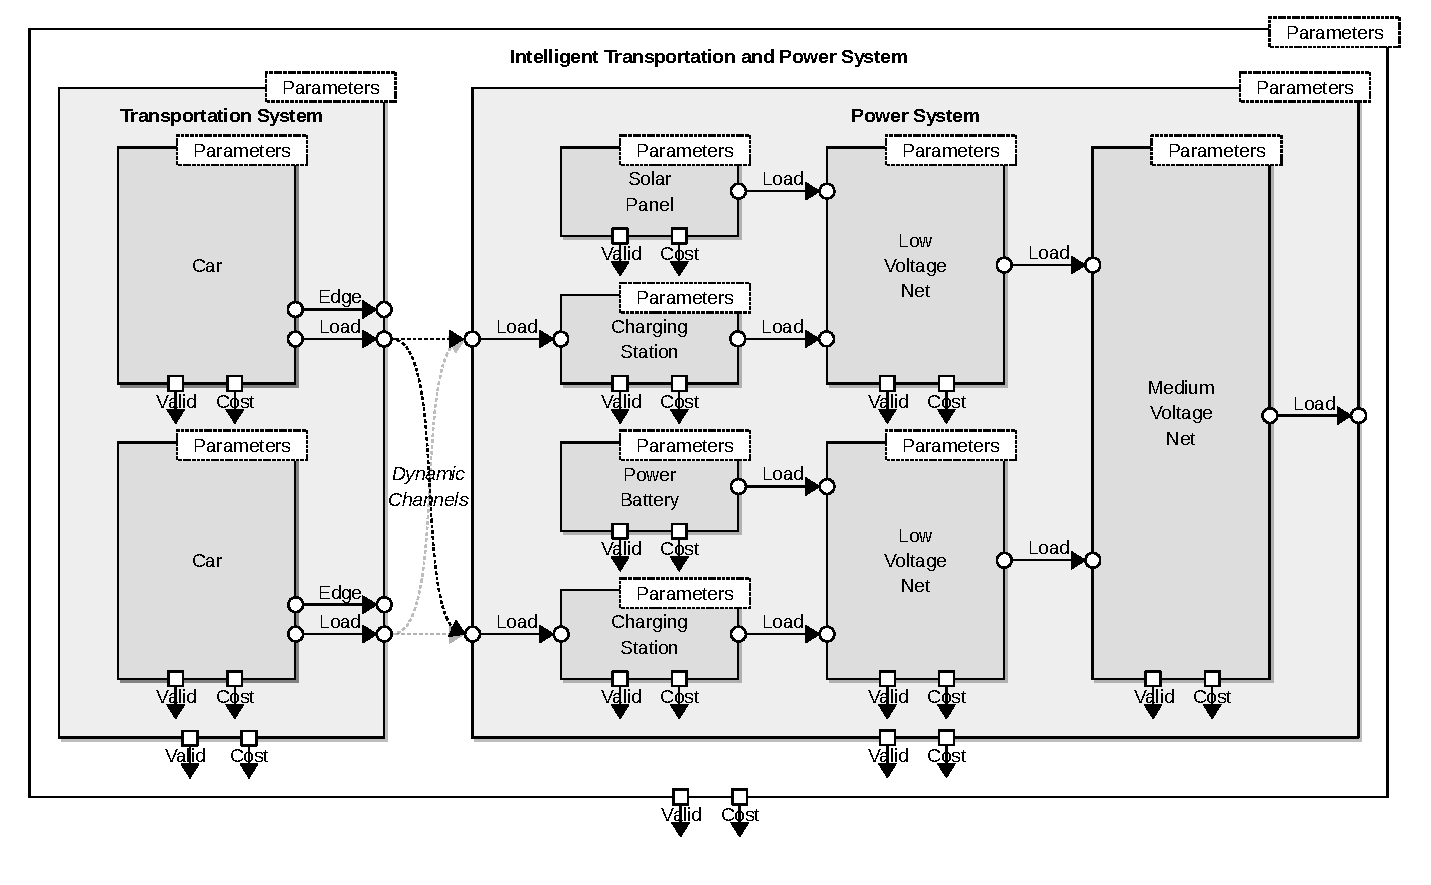
\includegraphics[width=\textwidth]{../gfx/model2.pdf}
	\caption{Overview of the multi-domain system modeling approach including the transportation system and the power system.}
	\label{fig:model}
\end{figure*}

\section{Holistic parametric approach (3 pages)}
\label{section:contribution_1}

In our approach, model definition is aided by a composite model architecture fitted to transportation scenario modeling seen in Figure~\ref{fig:model}. On it's highest level, the model architecture is represented by the intelligent transportation and power system model, which contains separate models for the transportation and the power system. The transportation model represents a transportation system, which is comprised of the individual cars within the traffic infrastructure. Similarly, the power model represents a power system, which is comprised of different energy producing or energy consuming power devices, such as solar panels, energy storages and charging stations. Furthermore, the power system includes electricity infrastructure such as low-voltage nets and medium-voltage nets. In terms of scenario definition, The employed approach to parametrization allows for components within the model to be initialized using a specific set of parameters. Parameterization allows for randomness in terms of the composition of individual components and their structure. The holistic parametric approach considers modeling and varying parameters of future transportation scenarios of both transportation and power systems.

Subsequently we shortly describe the different components of the model architecture in terms of their respective parameters, interface, structure and behavior.

\subsection{Intelligent Transportation and Power System}

The intelligent transportation and power system is a structure which contains the transportation and the power system.

\begin{table}[h]
	\renewcommand{\arraystretch}{1.3}
	\caption{Transportation System Component Parameters}
	\centering
	\begin{tabular}{lll}
		\hline
		\textbf{Parameter}                    & \textbf{Unit} & \textbf{Description} \\ \hline
		Traffic Network                  	  & Graph          & Graph of the traffic network      \\
		Transportation System                 & Component    & Contained transportation system    \\ 
		Power System                 		  & Component   & Contained power system    \\ \hline
	\end{tabular}
\end{table}

\subsubsection{Interface}

Inputs: Power System Load, Power System Cost, Transportation System Cost, Car Load, Car Position. Outputs: Cost, Validity, Balance, Car Load

\subsubsection{Structure}

Component composed of power system and transportation system components.

\subsubsection{Behavior}

The intelligent transportation and power system specifies a cost function which aggregates the costs of the transportation system and the electric network. On this cost function, a minimization objective is defined. Furthermore, the intelligent transportation and power system encodes dynamic channels between the output car loads of the transportation system and the input car loads of the power system. The output car loads of the transportation represent the source ports, while respective car positions of the transportation system represent source port options in each port/option pair. In return, input car loads of the power system and charging station positions of the power system are registered to the respective dynamic channels. Simply put, if a car's position matches a charging station's position while the car isn't driving, the power load of the car gets assigned to the power load of the charging station.

\subsection{Transportation System}

The transportation system is a structure representing the traffic infrastructure and the cars on the traffic infrastructure. Specifically, the transportation system is consisted of cars of different types, modeled as a distribution over multiple car types. The traffic infrastructure is modeled as a directed graph, whereby nodes represent reference points in the environment such as intersections, while edges in the graph represent road segments between these reference points. Nodes are defined by absolute position based on real-world coordinates, i.e. latitude, longitude, and elevation. Edges, i.e. road segments are defined through source and target node. Furthermore, edges are defined through an assigned number of lanes and a possessed road type, such as residential streets or highways.

\begin{table}[h]
	\renewcommand{\arraystretch}{1.3}
	\caption{Transportation System Parameters}
	\centering
	\begin{tabular}{lll}
		\hline
		\textbf{Parameter}              & \textbf{Unit}		 & \textbf{Description} \\ \hline
		Traffic Network                 & Graph          	 & Graph of the traffic network      \\
		Cars                  			& Numeral   		 & Number of cars      \\ 
		Car Distribution                & Numeral[]   		 & Distribution of different car types      \\ \hline
	\end{tabular}
\end{table}

\subsubsection{Interface}

Inputs: Car Cost, Car Load, Car Position. Outputs: Cost, Validity, Car Load

\subsubsection{Structure}

Component composed of car components.

\subsubsection{Behavior}

The transportation system specifies a cost function which aggregates the costs of the individual car components it contains. For this, the costs of individual cars are multiplied by the priority specified for individual cars. Then, secondly, these costs are aggregated to a single cost function. To ensure valid behavior, the transportation system implements a constraint on the car components which tests if cars overlap on their respective positions on the traffic network.

\subsection{Car}

Cars represent entities in the transportation system and on the traffic network. Fundamentally, they are defined by their origin and destination on the traffic network. In terms of physical representation, they are defined through their length and weight. Furthermore, they hold a battery of given capacity, i.e. the state of charge. Based on the battery, they encode rates defining the power transfer rate between car battery and charging stations.

\begin{table}[h]
	\renewcommand{\arraystretch}{1.3}
	\caption{Car Parameters}
	\centering
	\begin{tabular}{lll}
		\hline
		\textbf{Parameter}                    & \textbf{Unit} & \textbf{Description} \\ \hline
		Origin                                & Edge          & Origin Position      \\
		Destination                           & Edge          & Destination Position \\
		State of Charge Weight                & Numeral       & Weight of the state of charge objective                     \\
		Time Weight                           & Numeral       & Weight of the time objective                     \\
		Power Weight                          & Numeral       & Weight of the power objective                     \\
		Priority                              & Numeral       & Priority of the car in traffic                  \\
		Length                        	      & Metres        & Car length             \\
		Weight                        	      & Metres        & Car weight              \\
		State of Charge                       & kW/h          & State of charge of car battery                     \\
		State of Charge Minimum               & kW/h          & Allowed maximum for state of charge                    \\
		State of Charge Maximum               & kW/h          & Allowed minimum for state of charge                     \\
		Charge Rate Inflow                    & kW/h          & Maximum inflow while charging                     \\
		Charge Rate Outflow                   & kW/h          & Maximum outflow while charging                     \\
		Range Anxiety                         & Numeral       & Affinity to charge                     \\
		CS Selection Randomness 			  & Numeral       & Randomness of charging station selection                     \\ 
		Departure time 			  			  & Numeral       & Time to start traveling                    \\ \hline
	\end{tabular}
\end{table}

\subsubsection{Interface}

Inputs: -. Outputs: Cost, Validity, Load, Position.

\subsubsection{Structure}

Atomic component.

\subsubsection{Behavior}

When the departure time of a car is reached, it begins to travel from origin to destination. Origins, destinations and current position of a car are represented by edges on the traffic network.  When beginning to travel, a car's position is equivalent to the origin, while subsequent positions are selected from a determined route. Route and speed selection are determined non-deterministically based on the current position of the car. Specifically, route selection is based on a specified number of alternatives of shortest paths from the current position to the destination or the nearest charging station. Of these alternatives, one route is randomly selected. Furthermore, the route to the destination is dependent on the cars current state of charge. If the state of charge falls below a specified percentage described by it's range anxiety, the car route selection probability shifts the percentage specified by it's charging station selection randomness.

While traveling on the traffic network, cars consume energy based on traveled elevation profile, the car's mass and chosen speed. Within the car, energy consumption or production occurs based on the car's battery from which energy can be subtracted or can be added to. Energy consumption occurs while driving or while discharging the car's battery at a charging station. Energy production occurs through energy recuperation while driving or while charging the car's battery at a charging station. To ensure valid behavior, a constraint tests whether the battery's state of charge lies within a constant minimum and maximum level.
	
When connected to a charging station through a dynamic channel, charging occurs based on a probabilistic selection of states, which are uniformly distributed in terms of their probability. If the car choses to charge, a defined power load is transferred from the charging station to the car's battery. If the car choses to discharge, a defined power load is transferred from the car's battery to the charging station. Furthermore, the car can chose a zero state, in which no power load is transferred between car and charging station.
	
The objectives of a car's behavior are represented through multiple cost functions. Generally, costs of a car can only incur when it's departure time has been reached and are aggregated over time. Subsequently, we describe the underlying cost functions in detail. Firstly, a cost function for the car's convenience measures the cars state of charge in relation to the car's maximum state of charge. Secondly, a cost function for shortest traveling time aggregates the time needed for a car to reach it's destination. Thirdly, a cost function for the car's energy efficiency measures it's energy consumption in relation to the cars maximum energy consumption. The cost functions are aggregated and weighted by the impact of the different objectives by applying specific weights to the given cost functions.

\subsection{Electric Network}

The electric network is a structure representing the overall power system with the electric devices and infrastructure it contains.

\begin{table}[h]
	\renewcommand{\arraystretch}{1.3}
	\caption{Electric System Parameters}
	\centering
	\begin{tabular}{lll}
		\hline
		\textbf{Parameter}                    & \textbf{Unit} & \textbf{Description} \\ \hline
		Traffic Network                  	  & Graph          & Graph of the traffic network      \\
		Low Voltage Nets                          & Numeral    & Number of low voltage nets      \\
		LV Net Distribution                          & Numeral[]    & Distribution of LV net types      \\
		LV Net Allocation                          & Numeral    & Electric devices per LV net      \\   
		Medium Voltage Nets                        & Numeral    & Number of medium voltage nets      \\ 
		MV Net Distribution                          & Numeral[]    & Distribution of MV net types      \\
		MV Net Allocation                          & Numeral    & LV nets per MV net      \\   
		Solar Panels                       & Numeral    & Number of solar panels      \\ 
		Solar Panel Distribution                          & Numeral[]    & Distribution of solar panel types      \\  
		Charging Stations                          & Numeral    & Number of charging stations      \\
		CS Distribution                          & Numeral[]    & Distribution of charging station types      \\   
		Energy Batteries                        & Numeral    & Number of energy batteries      \\
		Energy Battery Distribution                          & Numeral[]    & Distribution of energy battery types      \\  \hline 
	\end{tabular}
\end{table}

\subsubsection{Interface}

Inputs: (Battery/Solar Panel/Charging Station/Low/Medium Voltage Net) Cost, Medium Voltage Net Load, Car Load. Outputs: Cost, Validity, Load, Car Load.

\subsubsection{Structure}

Component composed of battery, solar panel, charging station and low/medium voltage net components.

\subsubsection{Behavior}

The electric network specifies a cost function, which aggregates the costs of contained batteries, solar panels, charging stations as well as low and medium power nets. Furthermore, it aggregates the power loads of all medium voltage nets it contains to a single power load.

\subsection{Low/Medium Voltage Net}

Low- and medium voltage nets represent part of the electricity infrastructure. Based on a specific size, they can hold the power loads of different electric devices. Low- and medium voltage nets are limited in their ability to hold power loads through their capacity.

\begin{table}[h]
	\renewcommand{\arraystretch}{1.3}
	\caption{Low/Medium Voltage Net Parameters}
	\centering
	\begin{tabular}{lll}
		\hline
		\textbf{Parameter}                    & \textbf{Unit} & \textbf{Description} \\ \hline
		Balance Objective Weight       & Numeral    & Weight of the balance objective  \\  
		Size                  	  & Numeral    & Maximum number of devices/nets      \\
		Capacity          & kW/h    & Power load capacity      \\ \hline
	\end{tabular}
\end{table}

\subsubsection{Interface}

Inputs: (Battery/Solar Panel/Charging Station/Low Voltage Net) Load. Outputs: Cost, Validity, Load.

\subsubsection{Structure}

Atomic component.

\subsubsection{Behavior}

The low voltage net aggregates the power loads of all batteries, solar panels, charging stations it is assigned to a single power load. The medium voltage net aggregates the power loads of low voltage nets it is assigned to a single power load. Based on this aggregation, a cost function over the total power load balance is specified. The cost function is weighted by the impact of the balance objective by multiplying an according weight.

\subsection{Charging Station}
Charging stations are electric devices which act as power consumers or producers within the electric network and facilitate the charging process of the cars of the transportation system. They are assigned a physical location, i.e. specific position on the traffic network. The charging process is limited through a defined charge rate the charging station can relay to cars.

\begin{table}[h]
	\renewcommand{\arraystretch}{1.3}
	\caption{Charging Station Parameters}
	\centering
	\begin{tabular}{lll}
		\hline
		\textbf{Parameter}       & \textbf{Unit} & \textbf{Description} \\ \hline
		Position      			 & Edge    	     & Position on the traffic network of the charging station \\  
		Charge Rate         	 & kW/h    		 & Charge or discharge rate exposed to cars     \\ \hline
	\end{tabular}
\end{table}

\subsubsection{Interface}

Inputs: Car Load. Outputs: Cost, Validity, Load.

\subsubsection{Structure}

Atomic component.

\subsubsection{Behavior}

Charging stations can exhibit zero, negative or positive power load. Based on connection to a car, the charging station's behavior is determined by the selected charging state of the connected car. They act as energy consumers, when power load is transferred from the charging station to the connected car. Furthermore, they act as energy producers, when power load is transferred from the connected car to the charging station.

\subsection{Power Battery}
Power batteries represent electric devices which act as energy producers or energy consumers within the electric network.
This is attributed to their ability to consume and store or release energy given a specified battery power capacity. This ability is subject to loss of charge and to the battery's efficiency, which are applicable while charging and discharging. 

\begin{table}[h]
	\renewcommand{\arraystretch}{1.3}
	\caption{Power Battery Parameters}
	\centering
	\begin{tabular}{lll}
		\hline
		\textbf{Parameter}                    & \textbf{Unit} & \textbf{Description} \\ \hline
		State of Charge                       & kW/h          & State of charge of car battery                     \\
		State of Charge Minimum               & kW/h          & Allowed maximum for state of charge                    \\
		State of Charge Maximum               & kW/h          & Allowed minimum for state of charge                     \\
		Charge Rate                  	  	  & kW/h    	  & Battery (dis-)charge rate     \\ 
		Battery Loss                  	  	  & Numeral    	  & Loss of charge during (dis-)charging \\
		Battery Efficiency                    & Numeral    	  & Efficiency of (dis-)charge conversion     \\ \hline
	\end{tabular}
\end{table}

\subsubsection{Interface}

Inputs: -. Outputs: Cost, Validity, Load.

\subsubsection{Structure}

Atomic component.

\subsubsection{Behavior}

Based on probabilistic selection, the power battery chooses from different states determining energy consumption, production or zero load. In terms of their probability states are uniformly distributed. Energy consumption or production occurs based on the battery from which energy can be subtracted or can be added to. Energy consumption is caused by storing energy in the battery. Energy production is caused by releasing energy from the battery. To ensure valid behavior, a constraint tests whether the battery's state of charge lies within a constant minimum and maximum level.

\subsection{Solar Panel}

Solar panels are electric devices, which act as producers of renewable energy with a defined yield within the electric network. They are characterized by their situation related power production capabilities. This relation is approximated by a given mean of and variance of maximum power output within a given time.

\begin{table}[h]
	\renewcommand{\arraystretch}{1.3}
	\caption{Solar Panel Parameters}
	\centering
	\begin{tabular}{lll}
		\hline
		\textbf{Parameter}                    & \textbf{Unit}    & \textbf{Description} \\ \hline
		Power Scale                       	  & kW/h          	 & Maximum power output \\
		Mean                       	  		  & Numeral          & Mean for maximum power output  \\
		Variance                       	      & Numeral          & Variance for maximum power output \\ \hline
	\end{tabular}
\end{table}

\subsubsection{Interface}

Inputs: -. Outputs: Cost, Validity, Load.

\subsubsection{Structure}

Atomic component.

\subsubsection{Behavior}

Based on it's specific power scale, the solar panel produces an power load determined by mean and variance. Based on a probabilistic selection, the solar panel can choose to partially, fully or not dampen it's power load. The probability of these options is uniformly distributed.

\begin{figure*}[t]
	\centering
	
	\begin{subfigure}{\columnwidth}
		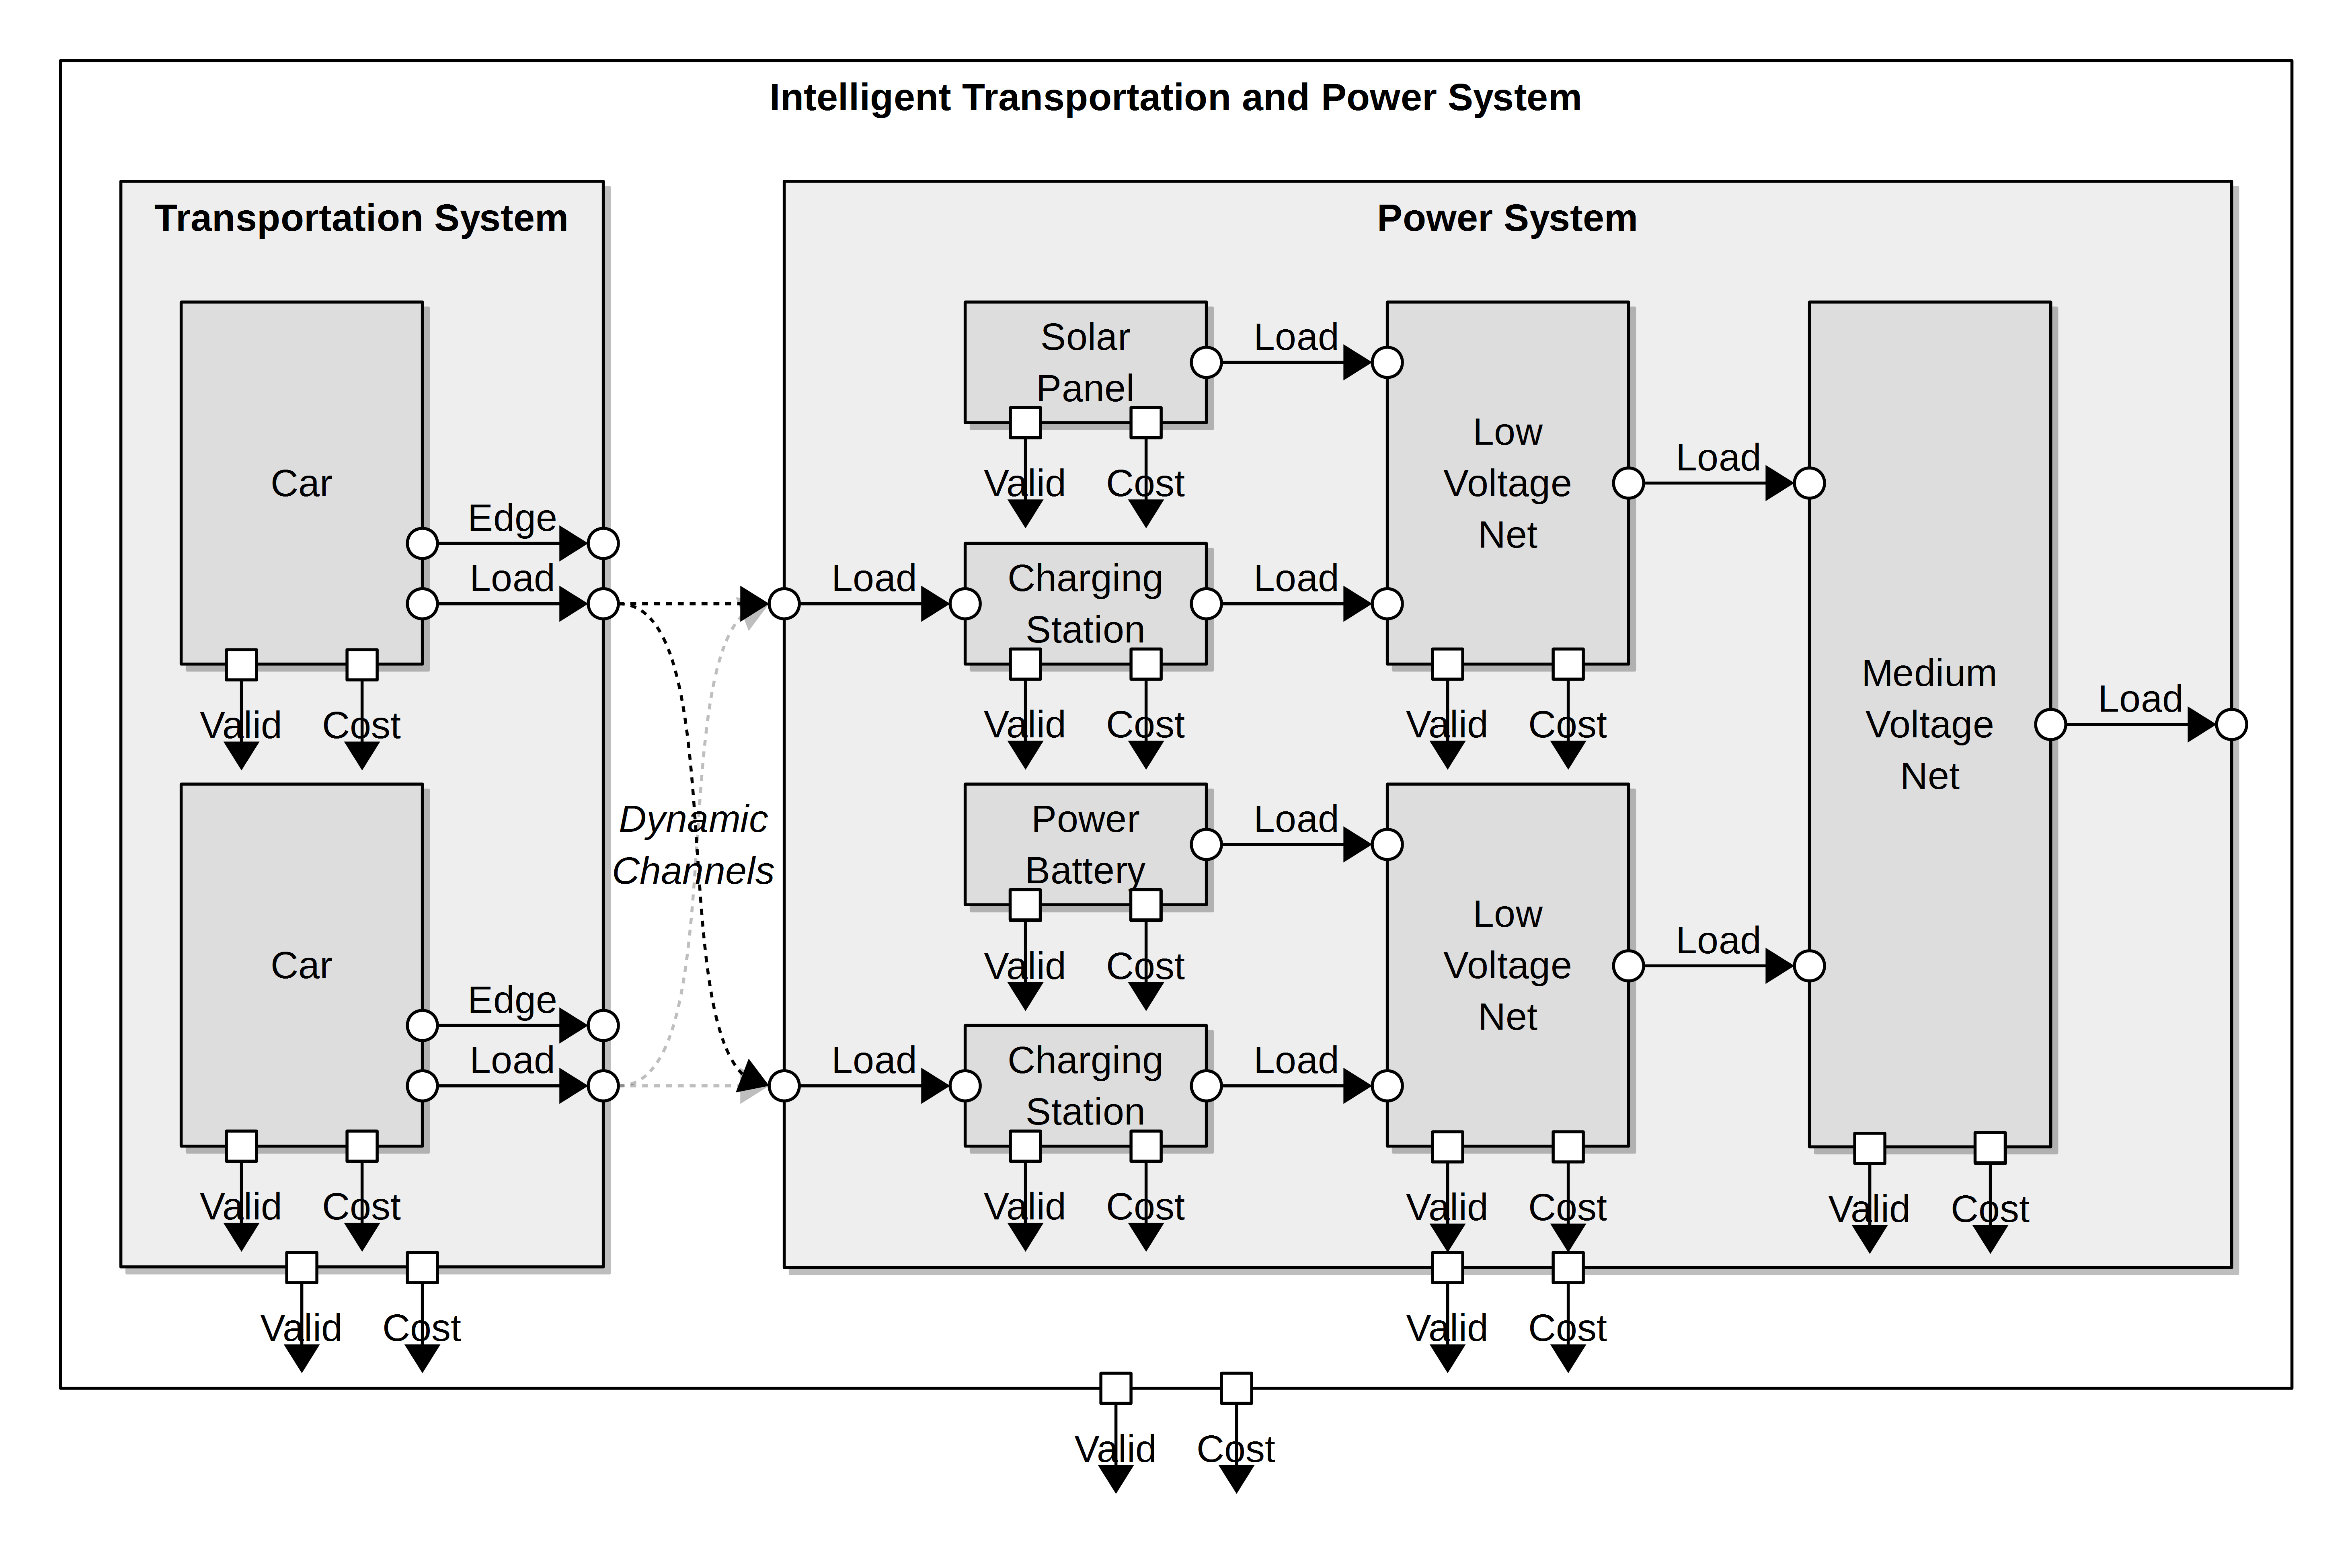
\includegraphics[width=\columnwidth]{../gfx/example.png}
		\caption{Example 1}
		\label{figure:examples_1}
	\end{subfigure}
	\hfill
	\begin{subfigure}{\columnwidth}
		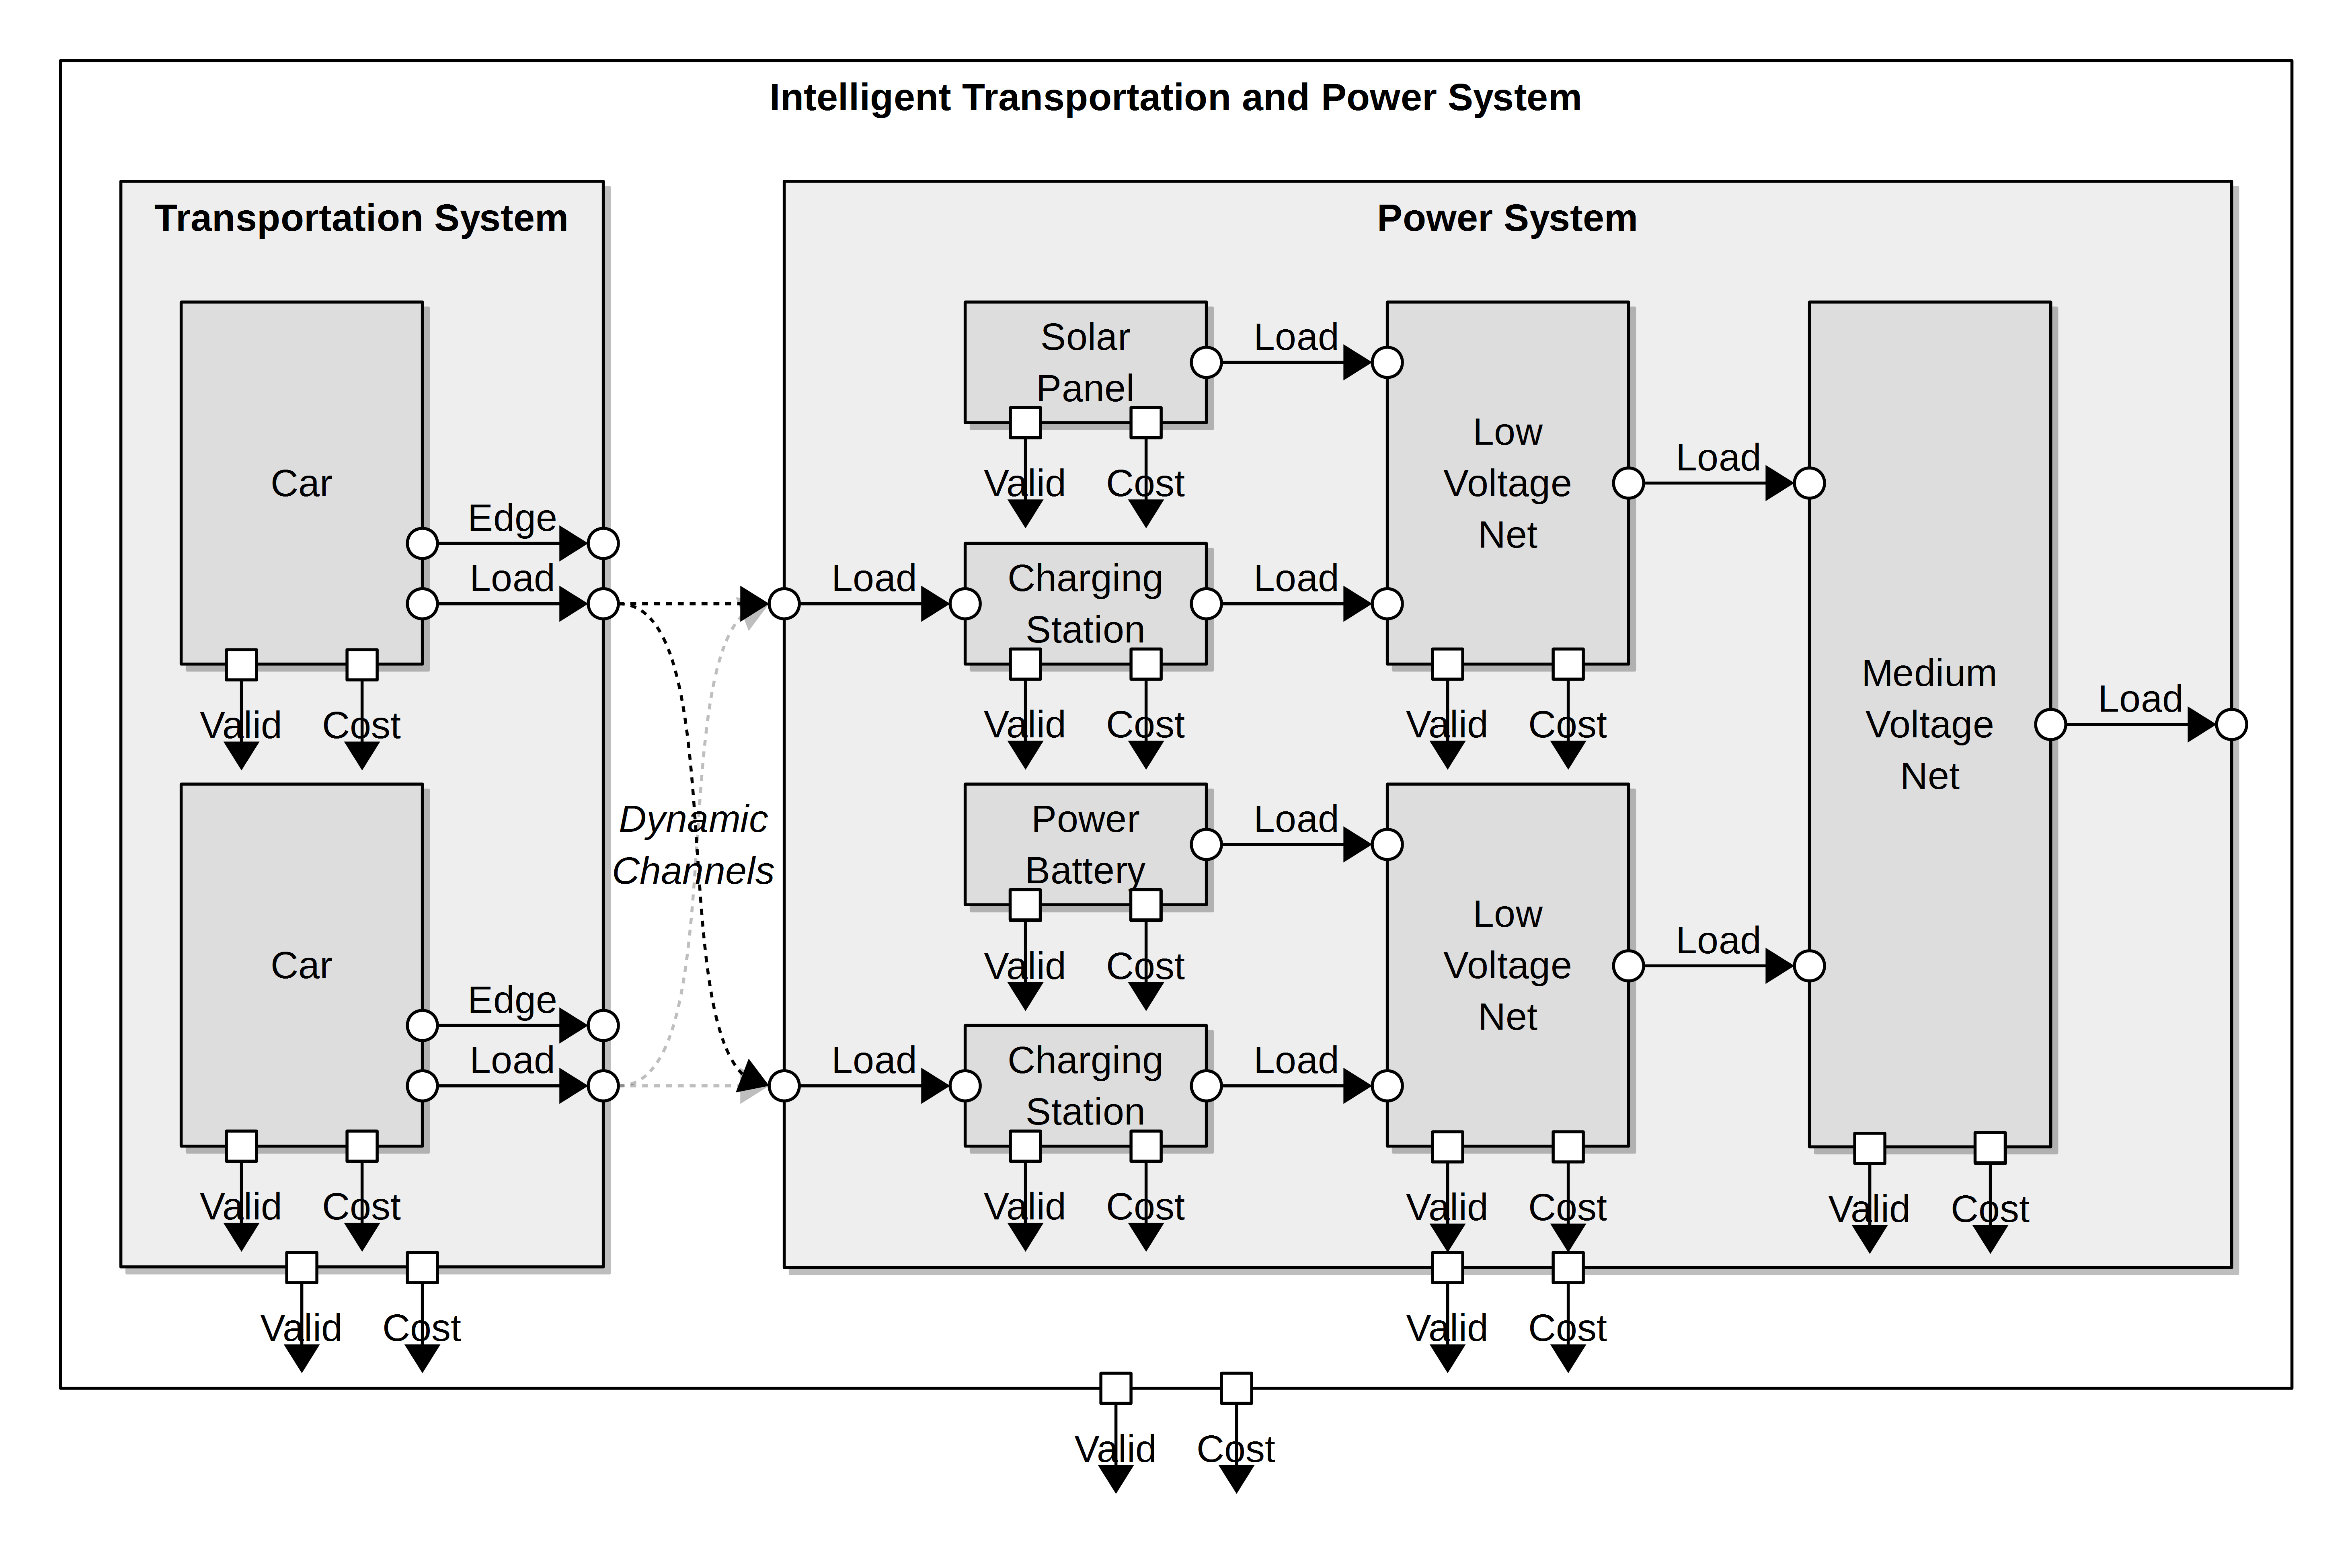
\includegraphics[width=\columnwidth]{../gfx/example.png}
		\caption{Example 2}
		\label{figure:examples_2}
	\end{subfigure}
	
	\begin{subfigure}{\columnwidth}
		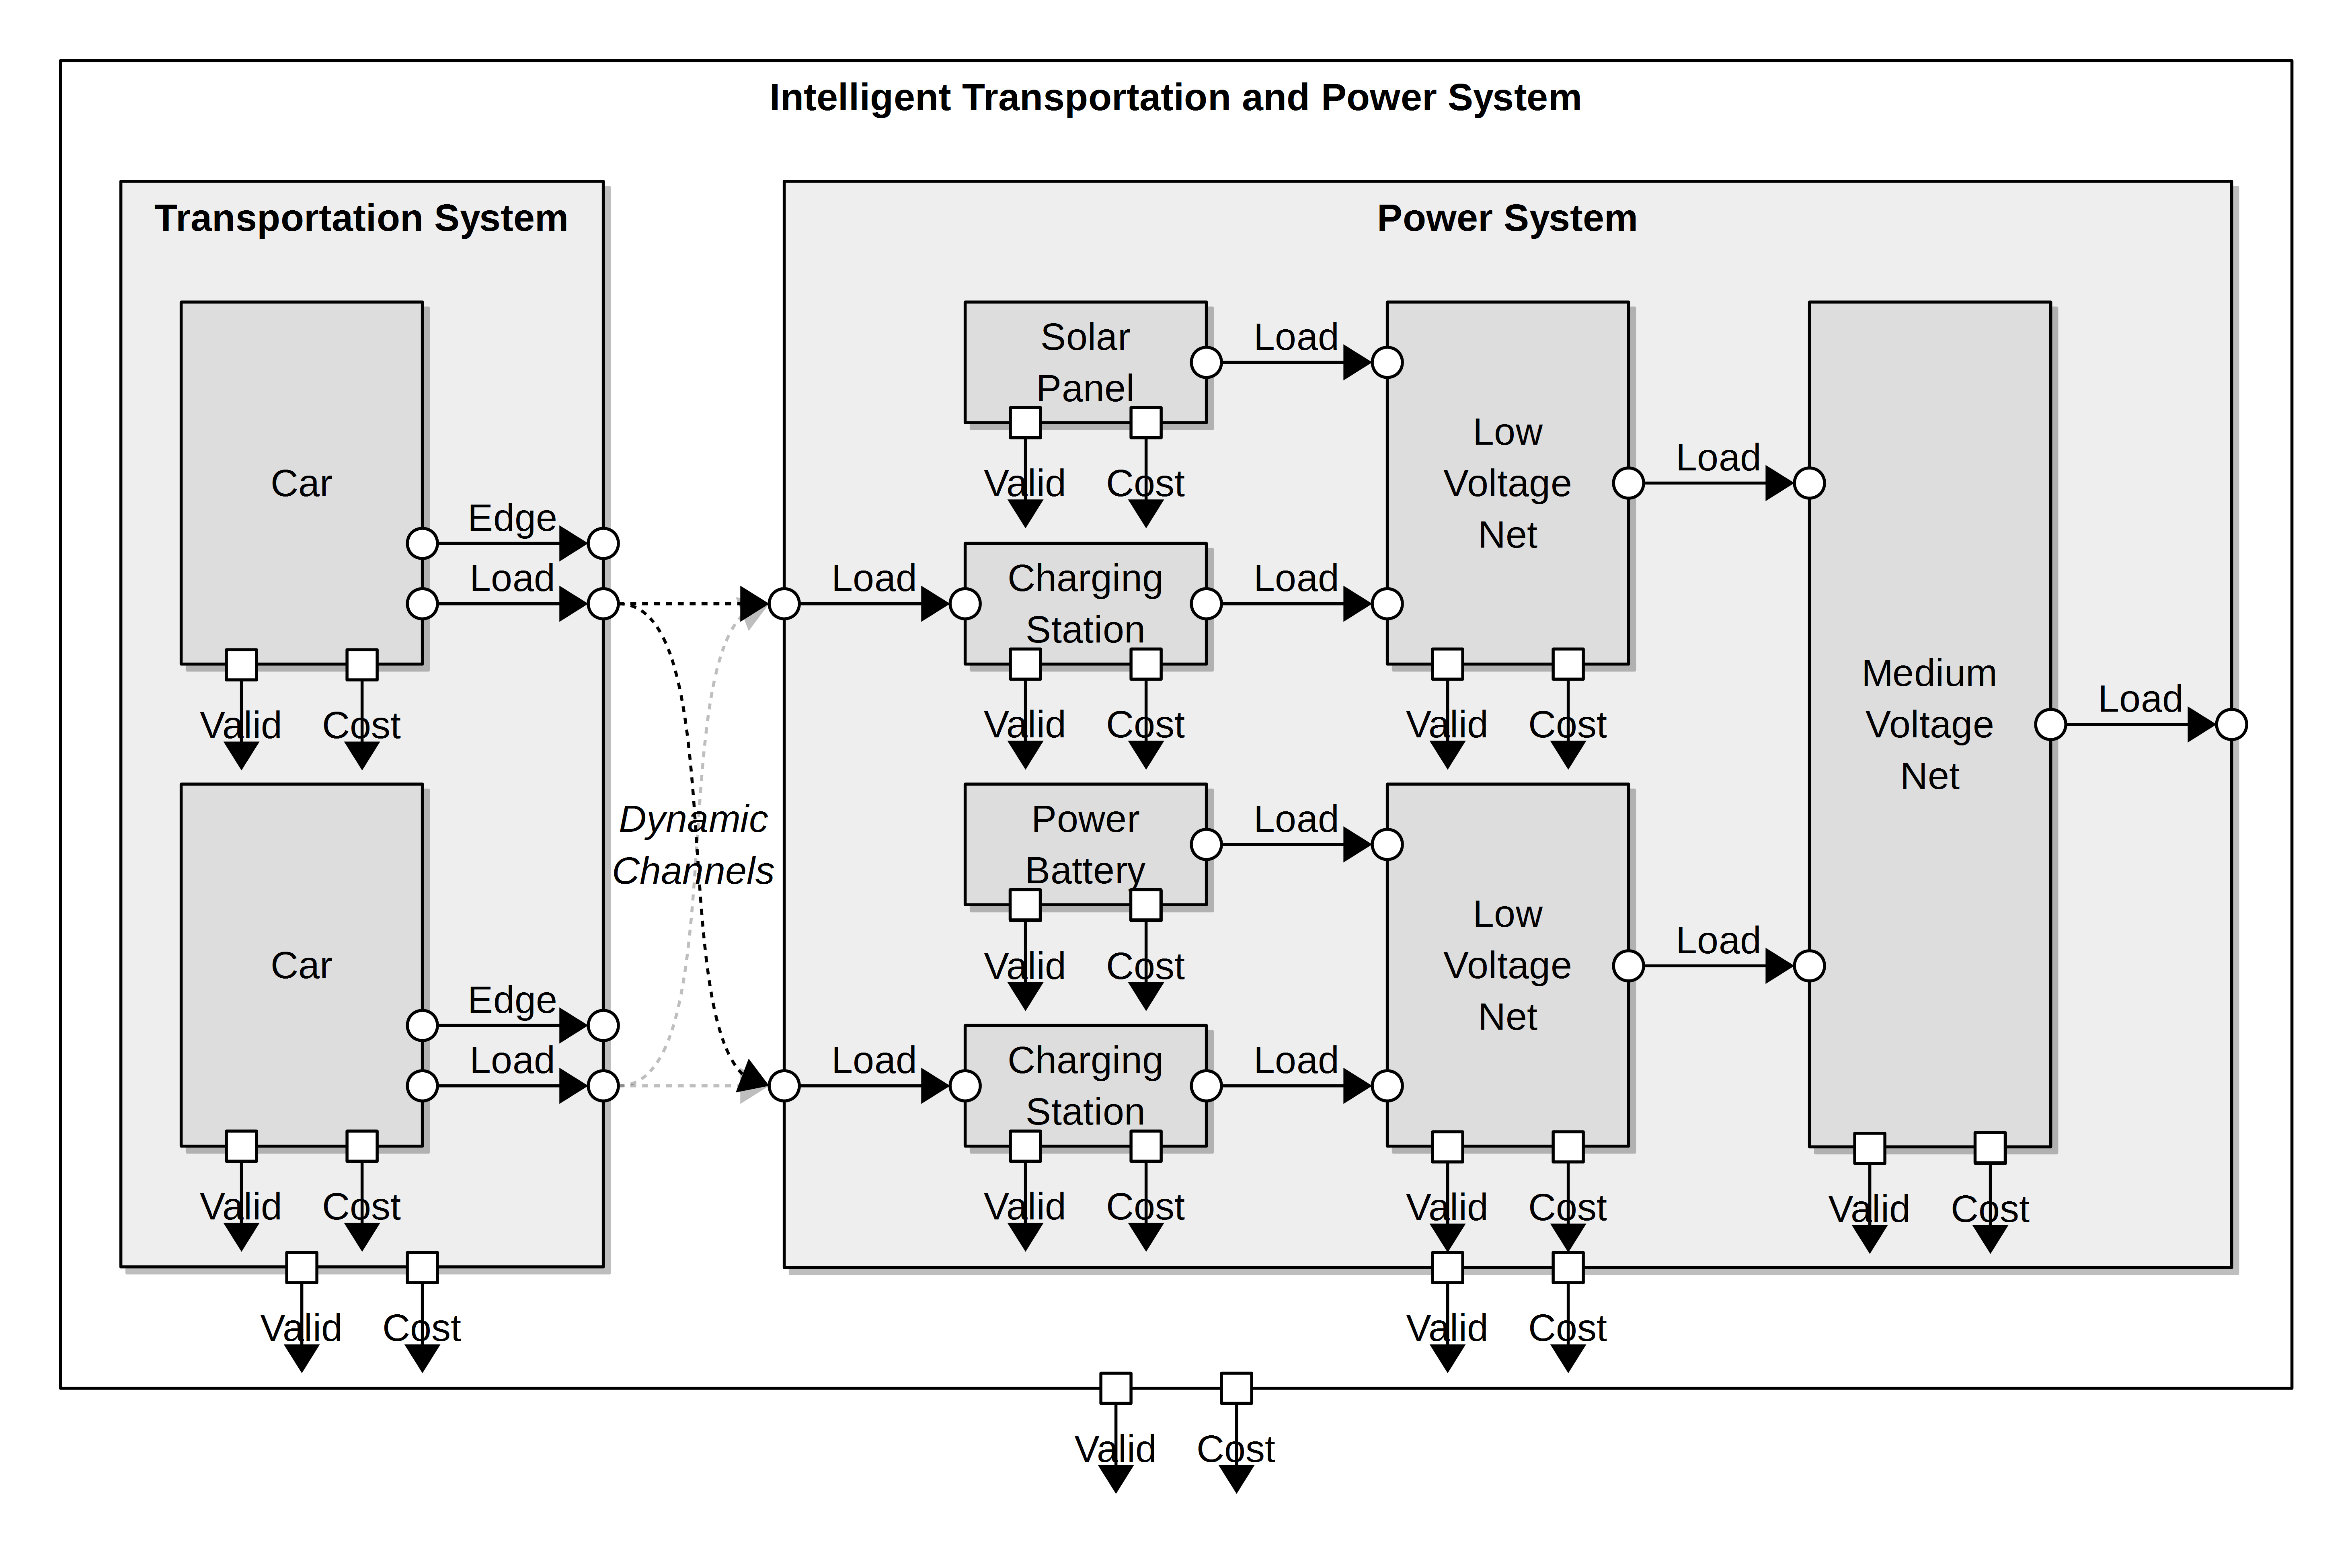
\includegraphics[width=\columnwidth]{../gfx/example.png}
		\caption{Example 3}
		\label{figure:examples_3}
	\end{subfigure}
	\hfill
	\begin{subfigure}{\columnwidth}
		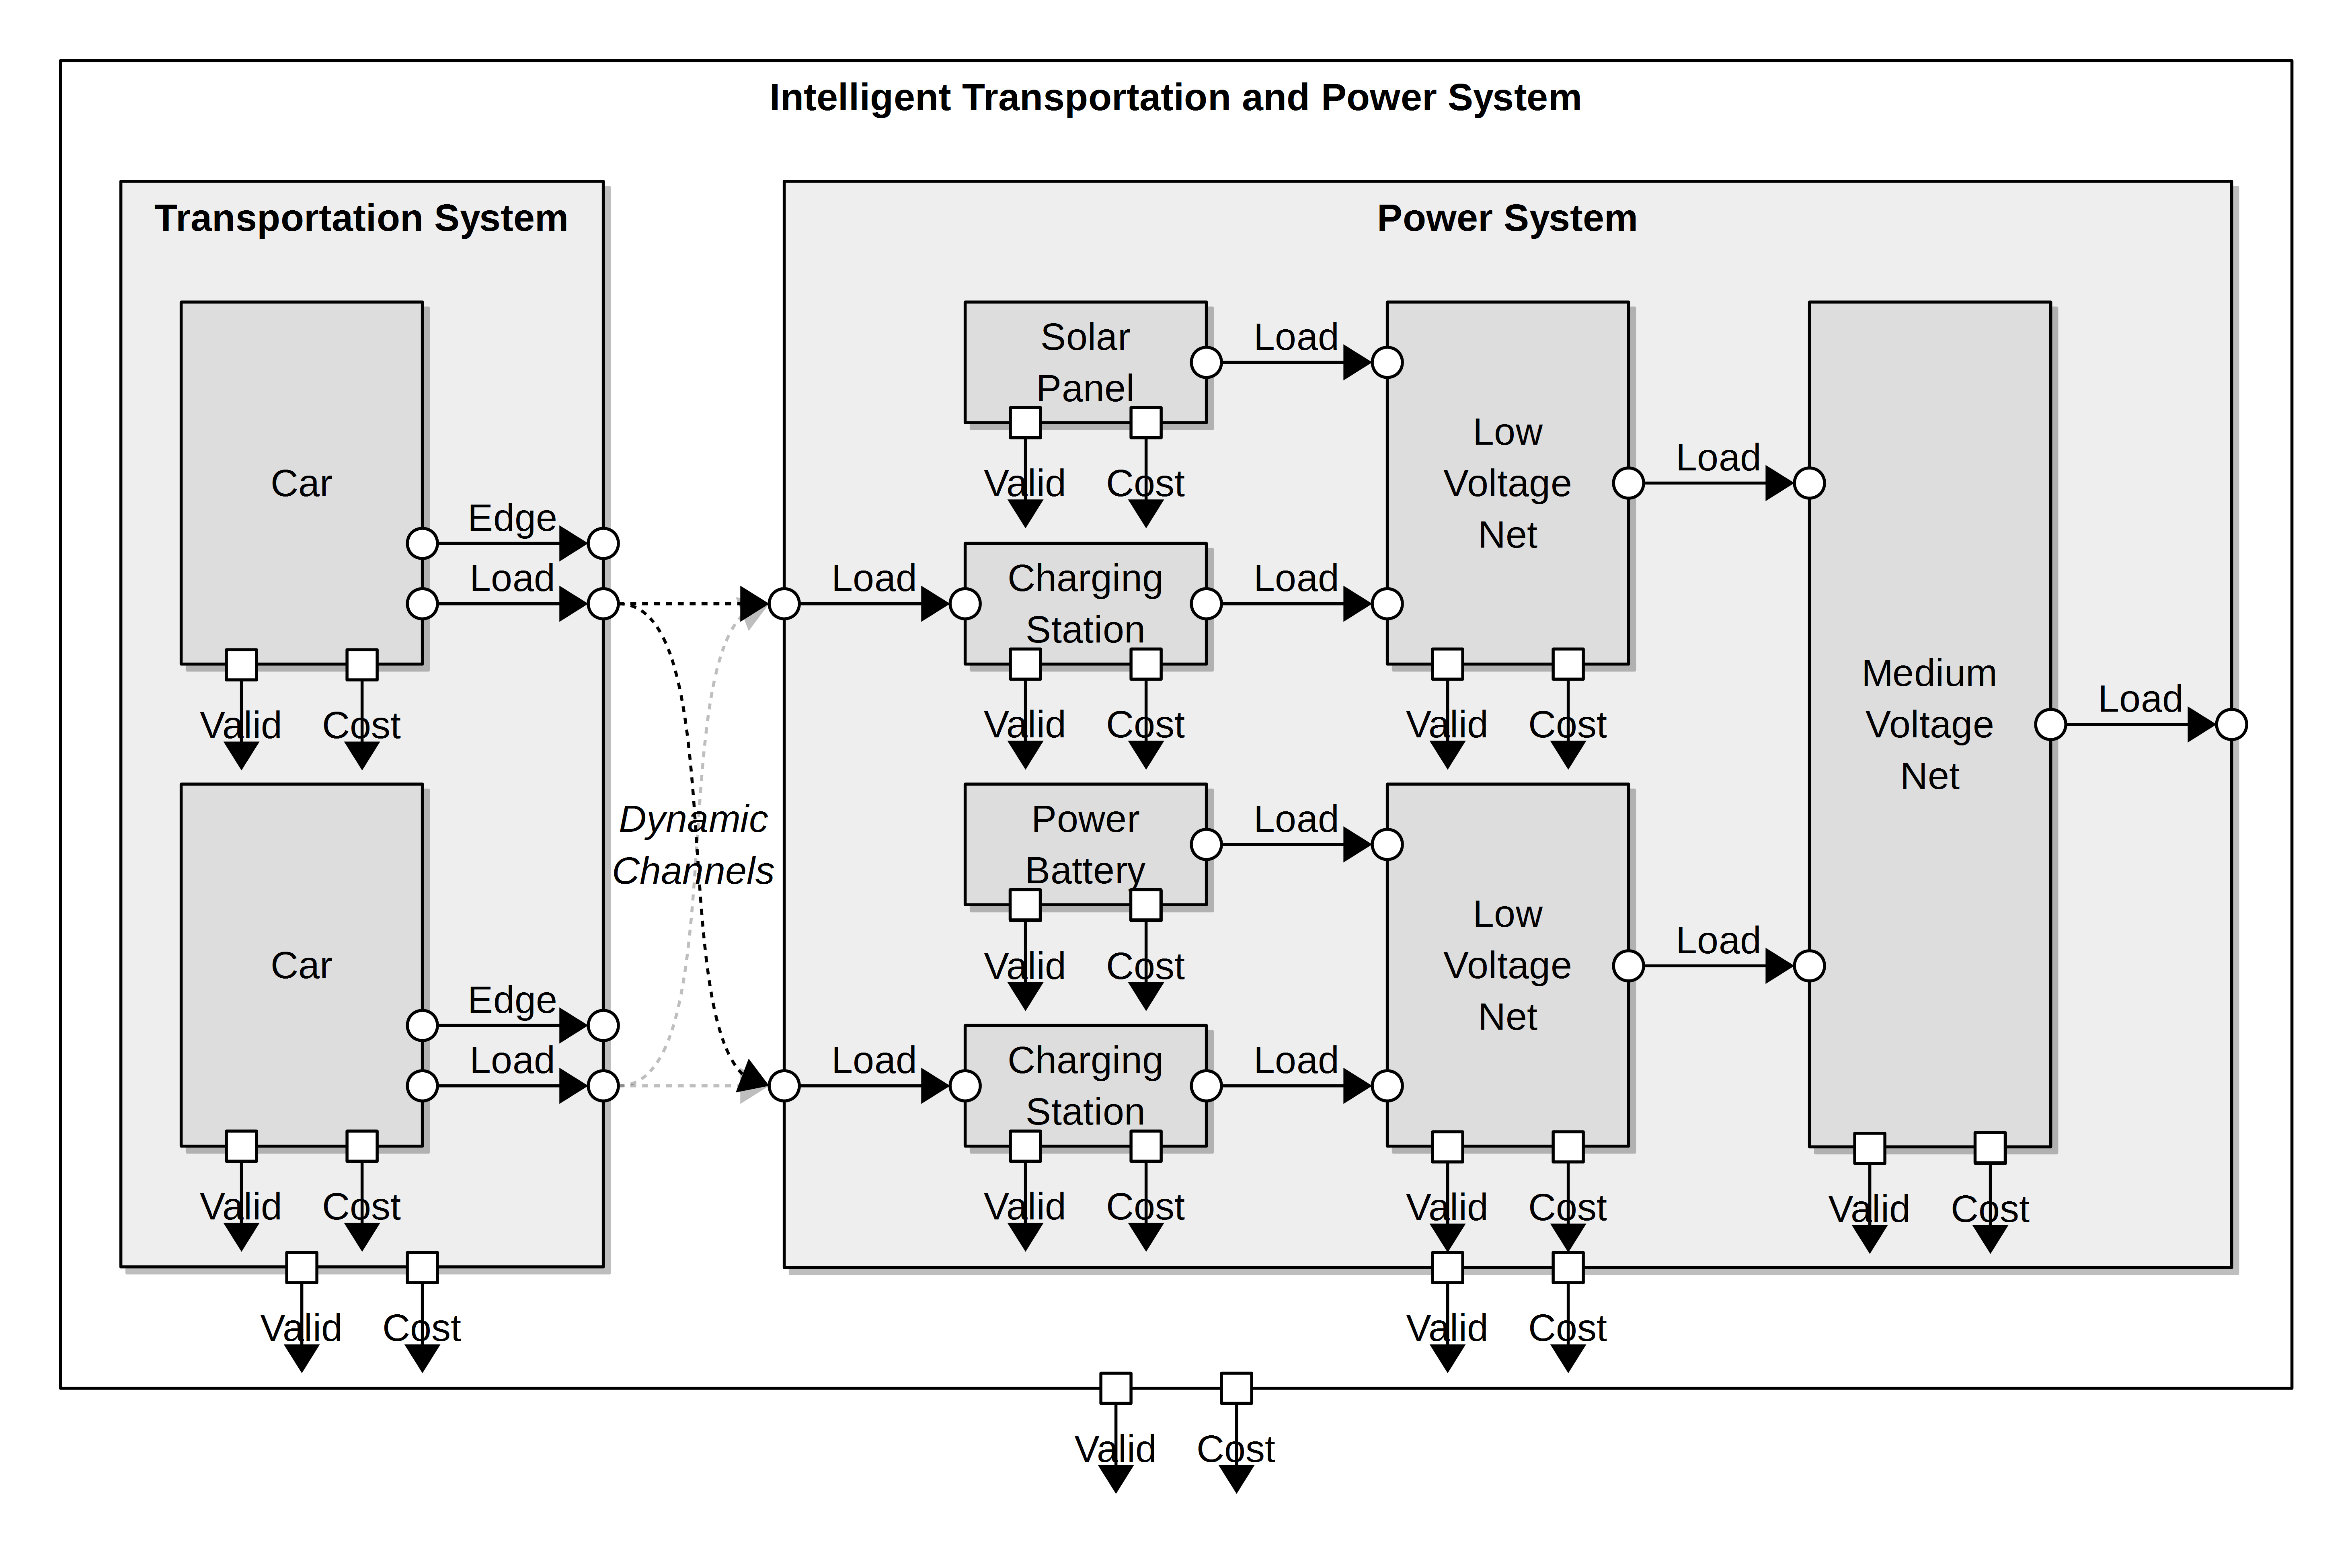
\includegraphics[width=\columnwidth]{../gfx/example.png}
		\caption{Example 4}
		\label{figure:examples_4}
	\end{subfigure}
	
	\caption{Examples.}
	\label{figure:examples}
\end{figure*}